\chapter{Storage: Architectures and Services}

\section{Evolution of the Storage Medium}
Storage represents the second fundamental pillar of a datacenter, the place where data persists across power loss (persistence). The absolute rule of storage is only one: \textbf{losing data is the unforgivable sin}.

\subsection{From Magnetic Tape to HDD and NVMe SSD}
Historically, the first datacenters used \textbf{Magnetic Tapes}: slow robotic cartridges but with enormous capacity and density. Tape forces a sequential access to data (you can't jump to the end without "unrolling" everything), but it is still used today for cold storage and offline backups impenetrable to ransomware (Air-gap).

\begin{figure}[H]
    \centering
    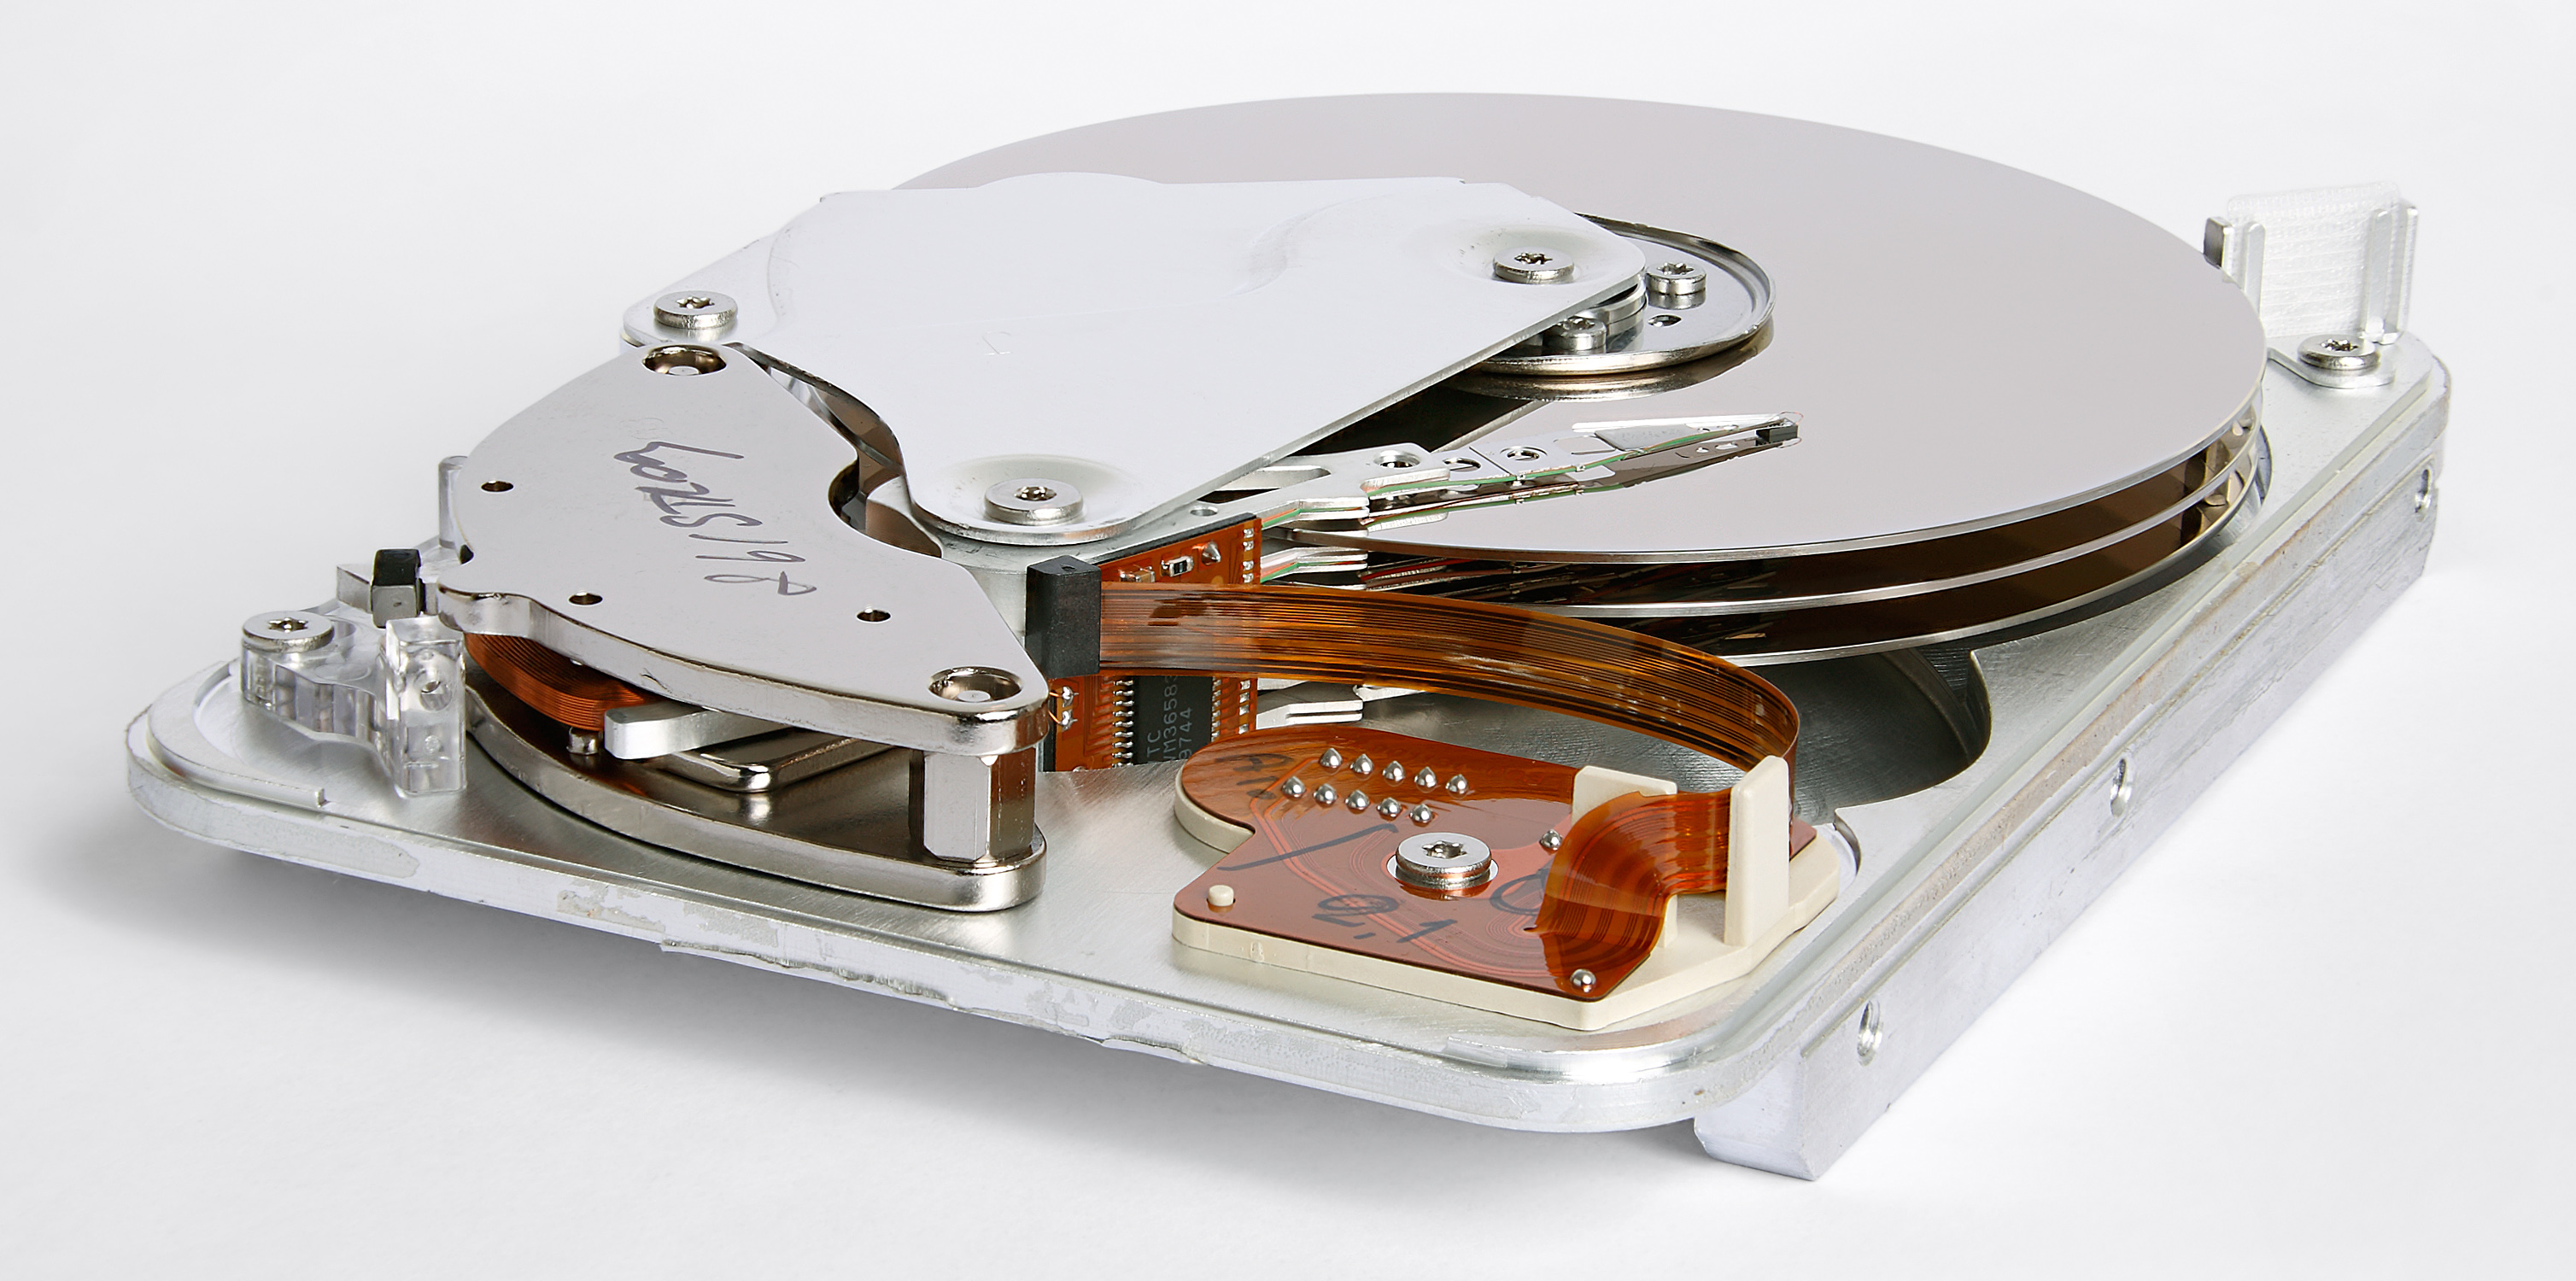
\includegraphics[width=0.6\textwidth]{images/hdd_inner.jpg}
    \caption{Inside a traditional mechanical magnetic Hard Disk Drive.}
\end{figure}
Subsequently, there was a shift to \textbf{HDDs (Hard Disk Drives)}, which offer random access to data. However, they are limited by mechanical constraints (rotation of platters, head \textit{seek} time), with impassable latencies of about 3-5 ms. Historical configurations for servers used complex cascaded interfaces (e.g., \textbf{SCSI}), today replaced by SAS or SATA protocols. Currently, HDDs are relegated almost exclusively to low-cost mass archiving.

The transition to \textbf{SSDs (Solid State Drives)} has reduced latency to a few hundred microseconds. However, the use of old SATA controllers quickly proved to be a bottleneck. The next revolution was the introduction of the \textbf{NVMe (Non-Volatile Memory Express)} standard, a protocol that connects flash memory directly to the \textbf{PCIe} bus, bringing latency down to $\sim$5-20 $\mu$s and throughput to tens of GB/s.

\begin{tipbox}[Modern Memory Hierarchy]
With NVMe, the performance gap between DRAM (nanoseconds) and permanent storage (microseconds) has shrunk from 6 to just 2 orders of magnitude, enabling software architectures unthinkable before, such as databases (e.g. RocksDB) that operate directly on storage without heavy caching layers in RAM.
\end{tipbox}

\subsection{NAND Cells and Asymmetry}
Unlike DRAM, NAND Flash memory has an intrinsic asymmetry: read operations are fast, while writes require a much slower PE (Program/Erase) cycle. The bit density per cell determines the type of SSD:
\begin{itemize}
    \item \textbf{SLC (Single-Level Cell):} 1 bit, extremely high endurance (100k PE cycles), extremely high cost.
    \item \textbf{MLC, TLC, QLC:} respectively 2, 3 and 4 bits per cell. Decreasing costs but rapidly declining endurance and write performance.
\end{itemize}

\begin{warningbox}[Data Retention and Over-provisioning]
Two critical engineering problems afflict modern SSDs:
\begin{enumerate}
    \item \textbf{Longevity (Data Retention):} To prevent the natural dissipation of electronic charge trapped in the cells, the SSD controller is forced to "silently" read and rewrite its NAND blocks in the background every $\sim$2 weeks. Without prolonged power (e.g., in Cold Storage), data on SSDs evaporates.
    \item \textbf{Over-provisioning:} An SSD cannot directly overwrite a block containing partial data; it must read, erase the entire block, and rewrite (Write Amplification). If an SSD exceeds 90\% capacity, the free space for these maneuvers (\textit{Garbage Collection}) runs out, causing a drastic and sudden drop in performance. To avoid this, pre-conditioning and hardware Over-provisioning are used (allocating a 10-20\% extra flash space at the factory that is invisible to the operating system).
\end{enumerate}
\end{warningbox}

\subsection{Performance Metrics: IOPS, Latency and Bandwidth}
Latency and Bandwidth (throughput) alone are not sufficient to characterize the performance of a storage system, as they depend heavily on the access pattern (sequential or random). 
A fundamental metric is \textbf{IOPS} (Input/Output Operations Per Second), which is the number of I/O operations completed in a second.
\begin{itemize}
    \item \textbf{Supermarket Analogy:} IOPS represents the customers served per second, latency is the time spent at the checkout for each customer, and parallelism (queues) are the open checkouts.
    \item The basic relationship for a single queue is: $\text{IOPS} \approx \frac{1}{\text{latency}}$.
    \item Thanks to the asynchronous nature of storage, protocols like NVMe (which support up to 64,000 parallel queues) allow to scale throughput immensely by processing many requests simultaneously.
\end{itemize}

\section{Aggregation and Protection: RAID and Resilience}
A single disk is an unacceptable single point of failure. \textbf{RAID} (Redundant Array of Independent Disks) is therefore used:
\begin{itemize}
    \item \textbf{RAID 0 (Striping):} No redundancy, extremely high performance, maximum risk.
    \item \textbf{RAID 1 (Mirroring):} Identical copy (Mirrored LUN), loses 50\% of the space but guarantees instantaneous availability in case of failure.
    \item \textbf{RAID 5:} Redundancy calculated via \textbf{XOR} logic function. Tolerance to the failure of only 1 disk. If a second disk fails during the delicate \textit{rebuild} phase (which can take days on modern large disks), all data is lost.
    \item \textbf{RAID 6:} Uses double parity, allowing the simultaneous failure of \textbf{2 disks}.
\end{itemize}

\textbf{The Twilight of Hardware RAID and Erasure Coding}\\
The advent of NVMe SSDs (with throughputs of tens of GB/s) has paradoxically rendered expensive \textit{Hardware RAID Controllers} obsolete. The controller chip cannot mathematically keep up with the parity calculation speed required for such fast disks, becoming the new bottleneck. Today, \textbf{Software RAID} dominates (e.g., \texttt{mdadm} on Linux or filesystems like ZFS), which delegates parity calculations to the immensely powerful multicore host CPUs.

In large-scale distributed cloud systems (like Object Storage), classic RAID fails. It is replaced by \textbf{Erasure Coding (n=m+k)}: a file is split into $m$ data fragments, to which $k$ mathematically calculated parity fragments are added. The fragments are scattered across tens of servers in different racks. It is possible to reconstruct the entire file having \textit{any} $m$ fragments available. This offers greater resilience than RAID at a lower storage cost, but with a higher CPU computational overhead.

\section{Storage Architectures in the Datacenter}

\subsection{SAN (Storage Area Network)}
SAN centralizes storage by separating it from servers, communicating at the block level (exposes raw disks, not files). The dominant protocols for this fabric are:
\begin{itemize}
    \item \textbf{Fibre Channel (FC):} Predominant legacy standard before the NVMe era, it relies on the \textbf{SCSI} protocol for block movement. It is a physically and logically separate network from standard Ethernet, often built with a physically redundant dual fabric topology (Fabric A and Fabric B). It requires dedicated cards on servers, called \textbf{HBA (Host Bus Adapters)}. It identifies nodes not by MAC addresses, but by 64-bit addresses called \textbf{WWN (World Wide Name)}.
    \item \textbf{iSCSI:} Economic alternative that transports SCSI commands inside normal TCP/IP packets over an Ethernet network. It works via a client-server architecture: the host server acts as an \textbf{iSCSI Initiator} (which requests blocks), while the storage array is the \textbf{iSCSI Target} (which provides them). Nodes are identified via \textbf{IQN} strings.
    \item \textbf{FCoE (Fibre Channel over Ethernet):} The historical attempt to unify the two networks. It encapsulates FC frames (SCSI) directly inside standard Ethernet (Lossless Ethernet using DCB/PFC protocols), eliminating the need for separate cabling, without the overhead of TCP/IP. Today it is almost entirely superseded by \textbf{NVMe-over-Fabrics (NVMe-oF)}.
\end{itemize}

\begin{tipbox}[SAN Security: Zoning and Masking]
To prevent one server from accidentally formatting (or intercepting the data of) another server's disk, two barriers are used:
\begin{enumerate}
    \item \textbf{Zoning (Network Side):} Applied on switches, it creates closed hardware zones. Similar to the concept of VLANs in Ethernet, it prevents two HBAs that are not in the same zone from communicating or "seeing" each other.
    \item \textbf{LUN Masking (Storage Side):} The storage array authorizes access to a logical disk (\textbf{LUN, Logical Unit Number}) exclusively to the specific WWN (for FC) or IQN (for iSCSI) address of the owner server.
\end{enumerate}
\end{tipbox}

\subsection{NAS (Network Attached Storage)}
NAS operates at a higher abstraction level, connected via standard Ethernet network (NFS or SMB protocols).
\begin{itemize}
    \item \textbf{Abstraction:} Exposes a logical File System (\textit{files and directories}).
    \item \textbf{Limits and mmap:} Higher network latency. In particular, NAS destroys application performance in case of massive use of the \textbf{memory mapping (mmap)} directive for random access (e.g. databases or VM virtual disk files). \textit{mmap} maps a logical disk file directly into the RAM space of a process (Page Cache). If the file resides remotely on a NAS, every single \textit{page fault} (reading a missing fragment in RAM) synchronously triggers an entire blocking Ethernet network round-trip, masking a disastrous I/O delay behind a simple memory instruction, leading to application stalls (\textit{stalls}). This problem does not occur with SAN block storage (direct DMA).
    \item \textbf{Use Cases:} File sharing, backups, corporate documents.
\end{itemize}

\subsection{Object Storage}
Developed to handle exabyte-scale scalability (e.g. Amazon S3). It abandons folders and blocks, using flat \textbf{objects} allocated in \textit{buckets} and queryable via REST APIs.
To ensure scalability and distribute data without a central bottleneck, it uses routing algorithms like \textbf{Consistent Hashing}. Ideal for massive static data, such as Machine Learning datasets or medical archives.

\subsection{HCI (Hyper-Converged Infrastructure)}
For decades the datacenter market was dominated by large vendors providing proprietary hardware SAN and NAS (e.g., the famous \textbf{EMC Symmetrix} arrays or \textbf{NetApp Filers}), extremely expensive appliances with difficult horizontal scaling. 
To cut costs and scale linearly, there was a shift to \textbf{HCI}, which transforms centralized SAN storage into a distributed approach (\textit{Scale-out}). Every server (commodity x86 node) contains CPU, RAM and local NVMe disks. A software layer (Software-Defined Storage) pools all local disks of all nodes and presents them to the hypervisor as a single large shared virtual SAN.
\begin{tipbox}[HCI Advantage]
\textbf{Data Locality:} The software always attempts to write/read the data of a VM in the disk physically residing in the same server that is running it, zeroing out North-South network traffic and fully exploiting local PCIe bandwidth.
\end{tipbox}

\subsection{Storage for AI: Vector Database}
The emergence of generative Artificial Intelligence required new storage paradigms. Classic textual search was purely \textit{syntactic} (like the \textit{bag of words} model), while neural models operate on \textit{semantics}.
\begin{itemize}
    \item \textbf{Embeddings:} Neural networks (LLMs) transform text, images or audio into very high-dimensional dense vectors (e.g. 3000 dimensions). These vectors, called \textit{embeddings}, represent the actual meaning of the data based on context (e.g., distinguishing "Python" as a language from "Python" as a snake).
    \item \textbf{Vector Database:} These are a new generation of NoSQL databases specifically designed to store and index these huge vectors. To answer a query, they vectorize the user's question and look for the most semantically similar documents by calculating the \textbf{cosine similarity} in the vector space.
\end{itemize}
\begin{tipbox}[RAG: Retrieval-Augmented Generation]
Vector Databases are the engine of the \textbf{RAG} architecture, an essential technique to limit AI "hallucinations". Before answering a prompt, the system queries the vector database, retrieves truly relevant corporate documents, injects them into the prompt, and forces the LLM to formulate the response based solely on those verified facts.
\end{tipbox}

\section{Advanced Services and Resilience}

\subsection{Efficiency: Deduplication, Compression and Tiering}
In addition to storing blocks, modern storage controllers (NAS/SAN) offer value-added services (often \textit{in-line}, computed in real-time during writing via dedicated ASIC chips):
\begin{itemize}
    \item \textbf{Deduplication:} Identifies and removes physically identical data blocks (e.g., if there are 100 Windows virtual machines with the same OS file, the data is saved only once on disk). A logical reference counter tracks the copies for the hosts.
    \item \textbf{Compression:} Mathematical reduction of the data footprint on disk.
    \item \textbf{Caching and Auto-Tiering:} Automatic promotion of the most read/written data blocks ("hot data") from slow disks to very fast tiers (e.g. NVRAM or NVMe SSD) completely transparent to the application.
    \item \textbf{Multipath I/O:} At the server level, each HBA is connected to parallel network fabrics (e.g., switch A and B) to have simultaneous logical paths to the same LUN of the storage array, ensuring load-balancing and instantaneous failover (MPIO).
\end{itemize}

\subsection{Snapshot, Thin Provisioning and Replication}
\begin{itemize}
    \item \textbf{Thin Provisioning:} Allows logically allocating more space to users than is physically present in the array, based on the principle that allocated space is rarely filled (\textit{Overbooking}). The fatal risk is physically exhausting free space if everyone writes, causing a systemic panic block of the entire datacenter (no one can write to disk anymore).
    \item \textbf{Snapshot vs Clone:} A \textit{Snapshot} is an instantaneous photograph of the volume at zero cost in terms of space. It exploits the \textbf{Copy-on-Write (COW)} mechanism: it freezes the original blocks and allocates new blocks (differential files) only for subsequent modifications. \textbf{Impact on performance:} a high chain of active snapshots heavily degrades read I/O performance. A \textbf{Clone}, instead, is a complete bit-by-bit physical copy (consumes space and time).
    \item \textbf{Crash-consistent vs Application-consistent:} A basic snapshot is always \textit{crash-consistent} (equivalent to brutally pulling the plug, without flushing RAM caches), which inevitably corrupts databases. To prevent this, the infrastructure uses agents like \textbf{Windows VSS (Volume Shadow Copy Service)} that coordinate with the OS to briefly "freeze" application I/O (\textit{quiesce}), take the snapshot and resume in an \textit{application-consistent} manner.
    \item \textbf{Synchronous/Asynchronous Replication:} Essential for Disaster Recovery. In the case of geographically close sites (within 15ms latency), \textbf{Metro Clusters} with synchronous active-active replication are used.
\end{itemize}

\subsection{Backup vs Replication}
\textbf{Replication} is a real-time mirror copy: it protects against hardware failures, but instantly propagates human deletions or ransomware attacks. \textbf{Backup} is a disconnected (offline) point-in-time save that allows recovery.

In the sizing of a business continuity system, two metrics are fundamental:
\begin{itemize}
    \item \textbf{RPO (Recovery Point Objective):} Amount of data the company is willing to lose (backup frequency).
    \item \textbf{RTO (Recovery Time Objective):} Maximum tolerable time for infrastructure recovery.
\end{itemize}

\begin{warningbox}[GDPR and Data Breach]
According to GDPR, a \textit{data breach} is not only the theft of data (loss of \textit{confidentiality}), but also includes the loss of \textit{integrity} (corrupted data) and \textbf{availability} (data intact but inaccessible, e.g. during a ransomware attack encrypting the only primary storage).
\end{warningbox}
